
\documentclass[journal,UTF8]{IEEEtran}
%\usepackage{ctex}
\usepackage{color}
\usepackage{diagbox}
\usepackage{booktabs}
\usepackage{cite}
\usepackage{threeparttable}
\ifCLASSINFOpdf
\usepackage[pdftex]{graphicx}
% declare the path(s) where your graphic files are
\graphicspath{{../pdf/}{../jpeg/}}
% and their extensions so you won't have to specify these with
% every instance of \includegraphics
\DeclareGraphicsExtensions{.pdf,.jpeg,.png}
\else
% or other class option (dvipsone, dvipdf, if not using dvips). graphicx
% will default to the driver specified in the system graphics.cfg if no
% driver is specified.
\usepackage[dvips]{graphicx}
% declare the path(s) where your graphic files are
\graphicspath{{../eps/}}
% and their extensions so you won't have to specify these with
% every instance of \includegraphics
\DeclareGraphicsExtensions{.eps}
\fi

\usepackage[cmex10]{amsmath}

%\usepackage{algorithmic}
\usepackage[ruled]{algorithm2e}
\usepackage{array}

\ifCLASSOPTIONcompsoc
\usepackage[caption=false,font=normalsize,labelfont=sf,textfont=sf]{subfig}
\else
\usepackage[caption=false,font=footnotesize]{subfig}
\fi

\hyphenation{op-tical net-works semi-conduc-tor}



\begin{document}
	%
	% paper title
	% can use linebreaks \\ within to get better formatting as desired
	% Do not put math or special symbols in the title.
	\title{VCA  Protocol-based Multi-level Flexible Architecture on Embedded PLCs for Visual Servo Control}
	
	\maketitle
	
	\begin{abstract}
		The visual system, motion control system, and programmable logic controller ($PLC$) system are becoming increasingly inseparable and important. However, their numerous types of programs and hardware, the many communication protocols among them, the mixed development methods, and the ever-growing high requirements and complexity lead to a cumbersome task of application implementation for users. Few works are researching the integration of these three systems to ease complexity. Most of them are focusing on their applications individually. 
		
		We propose herein a flexible multi-level architecture based on a vision control algorithm ($VCA$) protocol to decrease the complexity of ever-growing integrated applications. This multi-level architecture includes a flexible layer, a control layer, and an algorithm layer. The flexible layer is adopted to seamlessly integrate the visual system and the embedded PLC ($ePLC$). The $VCA$ protocol is designed for data interaction between the layers. Correspondingly, customized hardware, memory allocation, and Petri-Net-based multithreading structure are described to support the proposed flexible architecture. We implement two cases using the proposed $VCA$ protocol-based flexible architecture, in which the generality of the proposed flexible architecture is verified. In the first case, a winding machine with a visual system implements a regular winding effect by correcting $\theta$. In the second case, a binocular catching robot uses cameras to track the trajectory and send to $ePLC$. The robot can successfully catch the ball by adjusting the speed and the position. The cases indicate that the proposed $VCA$-based architecture could easily be applied between two different cases.
	\end{abstract}
	
	% Note that keywords are not normally used for peerreview papers.
	\begin{IEEEkeywords}
		embedded PLC, motion control, multi-level architecture, Petri Net, visual servo control
	\end{IEEEkeywords}
	
	% For peer review papers, you can put extra information on the cover
	% page as needed:
	% \ifCLASSOPTIONpeerreview
	% \begin{center} \bfseries EDICS Category: 3-BBND \end{center}
	% \fi
	%
	% For peerreview papers, this IEEEtran command inserts a page break and
	% creates the second title. It will be ignored for other modes.
	\IEEEpeerreviewmaketitle
	
	
	
	\section{Introduction}
	Integration technologies are driving industrial automation \cite{Kazmierkowski2007Integration}. The continuous integration of sensors, controllers, robots, tools, etc. has brought the concepts of self-aware equipment, intelligent factory, and cyber-physical system, among others \cite{Wan2018An,Chekired2018Industrial}. Recent studies  \cite{Colombo2006An,Vaccaro2010An,Dean2017Integration} introduced the development of integration technologies. In industrial automation, the $PLC$ system, motion control system, and visual system have become increasingly important and inseparable, as can be seen in various domains \cite{Chang2006Motion,Feng2005Practical}. %In addition, the advances of edge computing, fog computing, and edge artificial intelligence \cite{Hu2017Fog,Hou2018Green,PaceAn} put forward new challenges on edge equipment of these systems.
	
	\subsection{Motivations}
	Recent advances in image processing and pattern recognition contributed to the thriving of the visual system, which is being applied in various fields. The visual system could obtain parameters to replace the human visual system and address many tasks by extracting features from the image, especially the ever-growing requirements in industrial scenarios (e.g., works that should be finished in a dangerous environment, tasks that the human vision finds difficult to satisfy, and applications in some large-scale industrial productions, in which numerous visual systems are needed). 
	
	After visual processing, the motion control system, as the power of automation, is normally needed to drive some actuators to finish severe tasks, which remarkably benefits labor force replacement. 
	
	Furthermore, PLCs have become a base of automation because of their high reliability and easy programming \cite{Hossain2014Advanced}. Many studies are focusing on PLCs to extremely extend their applied fields. For instance, \cite{Jiang2013System} guaranteed reliability by verifying the program of PLCs; \cite{Dominic2016PLC} improved their performance using advanced algorithms; \cite{wu2018customized} alleviated their development complexity with a special software structure; and \cite{Sch2013Development} presented methods to dynamically update PLC programs.
	
	
	As mentioned before, the visual, motion control, and PLC systems are becoming increasingly inseparable. \cite{Chen2014A} described a typical case about how these three collaborate. The visual system analyzes the context and obtains error put into the motion control system. Simultaneously, the PLC analyzes information, such as the position limitation of every axis, to make some logical judgments accordingly. Regarding the normal development of these applications, the problems are met as follows:
	\begin{enumerate}
		\item The visual, motion control, and PLC systems are individually developed and combined using the communication protocol. However, this method should always be redesigned with the programs in these systems because of the difference of the visual and motion control algorithms and their organized logic programs. Moreover, many communication protocols (e.g., EtherCat, Modbus, CAN) are using these systems.
		\item The visual, logic, and motion control programs are always mixed together and developed within numerous visual systems, PLCs, and motion controllers, which increases the unnecessary complexity. 
		\item The requirements from customers are also increasing. Combined with the abovementioned two points, the development of corresponding applications has become a cumbersome task for developers. 
	\end{enumerate}
	
	Hence, how to pose a flexible structure for the integration of the visual, motion control, and PLC systems, which will ease the complexity, has attracted our interest.
	\subsection{Our Contributions}
	The contributions of our study are as follows:
	\begin{enumerate}
		\item We propose herein a $VCA$ protocol for generic data interaction between $ePLC$ and $VS$, which benefits the reuse of algorithms and the uniform use of communication protocols.
		\item A multi-level flexible architecture is posed for individual programming, which includes the flexible, control, and algorithm layers. Correspondingly, the customized hardware, memory allocation, and Petri-Net-based multithreading structure are described to support the proposed flexible architecture.
		\item The $VCA$ protocol-based multi-level flexible architecture implements further integration of the visual, motion control, and $PLC$ systems. The two implemented cases indicate that the proposed architecture could reduce the complexity of one application and from one to another.  
	\end{enumerate}
	
	The remainder of this paper is structured as follows: Section \ref{RW} introduces the related works; Section \ref{SystemStructure} presents the hardware and software structure and memory allocation; Section \ref{Integration} discusses the mechanism of the $VCA$ protocol in detail; Section \ref{Execution} illustrates the execution process of the proposed system; Section \ref{Case} presents the two implemented cases (i.e., binocular catching robot and winding machine with a visual system); and the last section concludes our work.
	
	\section{Related Works}
	\label{RW}
	The visual control system combined with the special motion control system and the visual system is applied in various fields, including the transportation \cite{Xing2014Intersection}, circuit detection\cite{Nian2005An}, sorting system, welding\cite{Chen2014A}, assembly\cite{Xiao2014Visual}, robotics\cite{Wu2013Cloud,Tsai2017A}, unmanned aerial vehicle\cite{Serra2016Landing}, and sorting\cite{Sun2013Automatic} fields. Works have addressed problems in relevant fields; however, all solutions are based on the special motion control and visual systems.
	
	The integration of logic control and motion control has also been presented in various deep studies\cite{Ioannides2004Design,Shi2016The,Fang2017Design}. \cite{Ioannides2004Design,syaichu2011model} directly realized motion control in the PLC. \cite{Qian2014A, OMRON2006CS1W} used a motion control module collaborated with the PLC to implement applications. However, it caused confusion as regards the development method in these works; hence, the PLCopen organization released a related standard \cite{PLCopen2005Function}, which standardized the motion control in the PLC. Based on this standardization, \cite{S2006Advanced} provided an advanced implementation in the distributed automation system, and companies, such as 3S \cite{3S2017Logic}, provided some tools for users. \cite{wu2018customized} also presented a customized real-time compilation method to reduce the development complexity.
	
	The abovementioned works have provided impressive integrations on the visual servo control system and the PLC with motion control functions; however, only a few works have investigated the integration of the visual, motion control, and PLC systems to decrease complexity. Most applications focus on their applications with three individual systems (e.g., \cite{Chen2014A}); hence, a further integration structure of the PLC that functions with motion control and the visual servo system should be provided to reduce the complexity and expand the application fields.
	
	
	
	\section{System Architecture}
	\label{SystemStructure}
	\subsection{Hardware Structure}
	Fig.\ref{fig:Hardware} shows hardware comprising $ePLC$ and the visual system ($VS$). The $ePLC$ is a customized structure. The number of digital input/output, analog input/output, and controlled servo system could be increased according to requirements. Particularly, the number of $ePLC$ processors could be customized for high-performance motion control applications. In motion control function-contained applications, more than two processors are always adopted, wherein one processor is mainly used for logic control, and the others are used for motion control. Fig. \ref{fig:Hardware} shows a typical $ePLC$, which adopts a two-processor architecture: a master and a slave processor. Shared memory is used for data interaction between the master and slave processors. The $VS$ normally contains one or more cameras and a processor for visual tasks. The communication between the $ePLC$ and the $VS$ could adopt multiple protocols, such as TCP, Modbus, and CAN.
	
	\begin{figure}
		\centering
		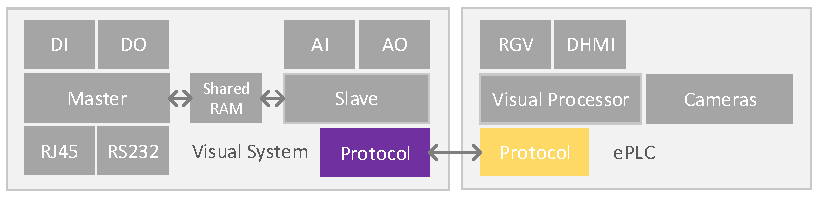
\includegraphics[width=3in]{fig/Hardware.pdf}
		\caption{Hardware architecture of the typical $ePLC$ and $VS$. The $ePLC$ adopts a two-processor architecture, while the $VS$ contains a camera and a processor. The communication between the $ePLC$ and the $VS$ adopts the CAN Bus.}
		\label{fig:Hardware}
	\end{figure}
	\subsection{Software Structure}
	Fig. \ref{fig:Software} shows software of the proposed multi-level flexible structure. To the best of our knowledge, the $VS$ commonly contains several visual algorithms, and every algorithm could extract some required parameters from pictures or videos. Meanwhile, the $ePLC$ comprises modules, which include logic part and algorithms. The algorithms here mainly denote the motion control algorithms. The structure contains three layers: flexible layer ($FL$), control layer ($CL$), and algorithm layer ($AL$).
	
	\textbf{Flexible layer}: This layer is responsible for joining the $VS$ and the $ePLC$ consisting of the $PLC$ interface and the visual interface. The parameters are framed with the $VCA$ protocol frame (henceforth, the $VCA$ protocol frame is the abbreviated form of $PF$) that interacted between the $VS$ and the $ePLC$. A special protocol template ($PT$) is also saved in both systems to illustrate the protocol.
	
	\textbf{Control layer}: This layer is separated from the algorithm layer to cope with the logic tasks, making it possible to run the logic task and the algorithm task in different processors.
	
	\textbf{Algorithm layer}: This layer mainly comprises various types of algorithms. The independent algorithm layer allows the algorithms to achieve a high-performance requirement that could be built in individual processors. 
	
	
	\begin{figure}
		\centering
		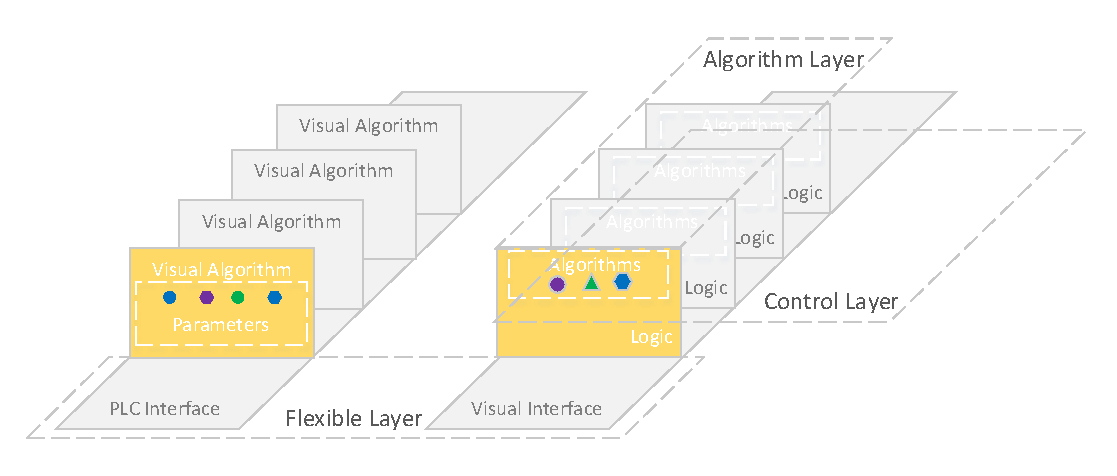
\includegraphics[width=3in]{fig/Software.pdf}
		\caption{The multi-level flexible architecture contains three layers: flexible, control, and algorithm layers. The $VS$ contains several visual algorithms used to extract parameters from pictures or videos. The flexible layer consists of the PLC interface and the visual interface used to combine the $ePLC$ and the $VS$. The control layer is mainly designed for the logic program. The algorithm layer comprises many algorithms, and every algorithm has several parameters.}
		\label{fig:Software}
	\end{figure}
	
	
	\subsection{Memory Allocation}
	\begin{figure}
		\centering
		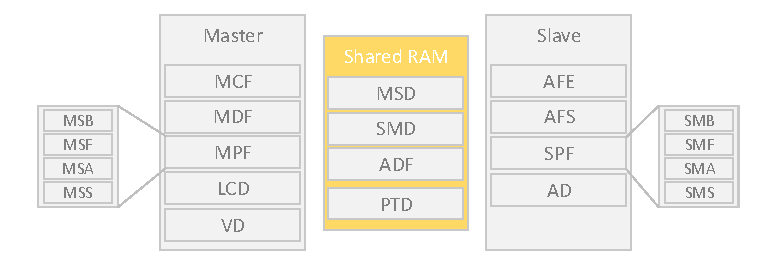
\includegraphics[width=3in]{fig/RAM.pdf}
		\caption{Memory allocation of the master processor, shared RAM, and slave processor.}
		\label{fig:RAM}
	\end{figure}
	The dedicated storage area of the $ePLC$ in the memory is made up of the bit data area ($M$ area) and the byte data area ($D$ area). We regard the $M$ and $D$ areas as the set $M$ of bit and the set $D$ of byte, respectively. Henceforth, if set $S$ $\exists$, we define its subscripted lowercase letter $s_i$ as an element of $S$, and the subscripted $i$ is used to distinguish the elements. Fig. \ref{fig:RAM} shows the memory allocation of the master processor, shared RAM, and slave processor according to hardware of Fig. \ref{fig:Hardware}. The shared $RAM$ is a special structure for the fast data interaction between the master and slave processors. In more general cases, the $MSD$ is located in the master processor; $SMD$ and $ADF$ are located in the slave processor; and $PT$ is in both the master and slave processors. 
	
	The RAM in the master processor contains special areas: 1) the module control flag area ($MCF$) is used to start the modules; 2) the master processor data interaction flag area ($MPF$) contains the begin data transfer flag from master to slave ($MSB$), transferring the state of master from master to slave ($MSF$), acknowledging flag of master from master to slave ($MSA$), and transferring the state of master from slave to master ($MSS$); 3) the module data saved flag area ($MDF$) denotes whether the module data are saved; 4) the logic control data area ($LCD$) is used to store the control frame, where every element $lcd_i$ is associated with a specified module; and 5) the $VCA$ protocol frame data area ($VD$) stores all the frames received from the $VS$.  
	
	In the shared RAM, it could be read by both the master and slave processors and consists of special areas: 1) the master processor data interaction data area ($MSD$) stores the data delivered from the slave processors; 2) the slave processor data interaction data area ($SMD$) stores the data delivered from the master processor; 3) the algorithm data saved flag area ($ADF$) denotes whether the algorithm data are saved; and 4) the protocol template data area ($PTD$) stores the protocol template containing the $PT$s from the $VS$ to the $ePLC$ and from the $ePLC$ to the $VS$.
	
	
	In the slave processor, the RAM comprises special areas: 1) the algorithm flag area ($AF$) includes the algorithm flag of execution ($AFE$) and the algorithm flag of state ($AFS$); 2) the slave processor data interaction flag area ($SPF$) includes the begin data transfer flag from slave to master ($SMB$), transferring the state of slave from slave to master ($SMF$), acknowledging flag of slave from slave to master ($SMA$), and transferring the state of slave from master to slave ($SMS$); and 3) the algorithm data area ($AD$) saves data that help in the specified algorithm execution.
	
	We define $\mathcal{I}$ for the data interaction between the master and slave processors, and it contains two parts: transferring data from master to slave ($\mathcal{I}_{mts}$) and transferring data from slave to master ($\mathcal{I}_{stm}$):
	\begin{equation}
	\left\{
	\begin{array}{l}
	\mathcal{I}_{mts} = \mathcal{L} (msb_i,msf_i,sma_i,sms_i,smd_i),\\
	\mathcal{I}_{stm} = \mathcal{L} (smb_i,smf_i,msa_i,mss_i,msd_i),
	\end{array}
	\right.
	\end{equation}
	where $\mathcal{L}$ is the function to implement the data interaction process between the master and slave processors. $\mathcal{I}_{mts}$ and $\mathcal{I}_{mts}$ use the same function $\mathcal{L}$. The $\mathcal{I}_{mts}$ process is described as follows: the master processor sets $msb_i$ to one, sets $msf_i$ to one, sends data to $smd_i$, recovers $msb_i$ to zero, and informs the slave processor to obtain the data; the slave processor sets $sms_i$ to one, checks the data of $msd_i$, sets $sma_i$ to one, feeds back the master processor to end the transferring, recovers $sms_i$ to zero, and recovers $sma_i$ to zero; and the master processor recovers $msf_i$ to zero. 
	
	
	%%%Fig.6. Distribution of dedicated public data area.
	\section{Integration of $VS$ and $ePLC$}
	\label{Integration}
	
	\subsection{$VCA$ $PT$}
	\begin{figure}
		\centering
		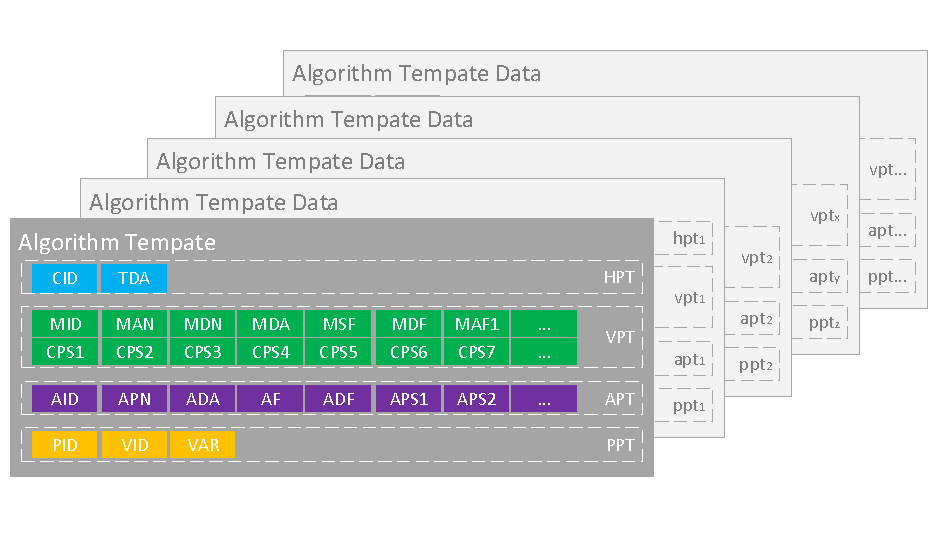
\includegraphics[width=3in]{fig/PT.pdf}
		\caption{A $PT$ uniquely corresponds to a type of application and contains four parts: head of the protocol template, visual layer template, control layer template, and algorithm layer template.}
		\label{fig:PT}
	\end{figure}
	For most applications, we design the $VCA$ protocol for data interaction among the layers. As shown in Fig. \ref{fig:PT}, a protocol template ($PT$) was adopted to support various types of implementations, and the $PT$ uniquely corresponded to a type of application. In the flexible architecture, the users only needed to redesign and reload the $PT$. They can then reuse the visual servo system. The $PT$ could be loaded into a stationary address of the visual and $ePLC$ systems. After restarting both systems, it will be stored into a fixed area of the $RAM$. The parsing modules from both systems will read it when parsing the $PF$. The $VCA$ protocol could be used to bidirectionally transfer the $PF$ using the same $PT$ and algorithms of framing and deframing.  
	
	$PT$ is defined below:
	\begin{equation}
	\left\{
	\begin{array}{l}
	PT = \{HPT, VPT, APT, PPT\}\\
	HPT = \{CID, TDA\}\\
	VPT = \{MID, MAN, MDN, MDA, MSF, MDF, \\
	\qquad\qquad\quad \bigcup_{x=1}^i MAF_x, \bigcup_{x=1}^j CPS_x\}\\
	APT = \{AID, APN, ADA, AF, ADF, \bigcup_{y=1}^i APS_y\}\\
	PPT = \{PID, VID, VAR\}
	\end{array}
	\right.
	\end{equation}
	
	
	The $PT$ contains four parts: head of the protocol template ($HPT$), VCA protocol template ($VPT$), algorithm protocol template ($APT$), and parameter protocol template ($PPT$). Every part is explained below:
	\begin{enumerate}
		\item $HPT$: This part includes a communication unique ID ($CID$) and a template data storage address ($TDA$). Every $PT$ only has one $HPT$.
		\item $VPT$: This part consists of a module unique ID ($MID$), a module contained algorithm number ($MAN$), a module contained data number ($MDN$), a module data start address ($MDA$), a module start flag ($MSF$), a module data saved flag ($MDF$), and module contained algorithm IDs ($MAS_x$). $VLT$ is not $\emptyset$. Every $VPT$ includes $MAN$ algorithm IDs. 
		\item $APT$: This comprises an algorithm unique ID ($AID$), an algorithm contained parameter number ($APN$), an algorithm data start address $ADA$, an algorithm data saved flag ($ADF$), and an algorithm contained parameter IDs ($APS_y$). $CLT$ is not $\emptyset$. Every $APT$ includes $APN$ parameter IDs.
		\item $PPT$: This contains a parameter unique ID ($PID$), its relevant visual algorithm ID ($VID$), and the conversion ratio of the visual and motion algorithm parameters ($VAR$).  
	\end{enumerate}
	\subsection{$VCA$ $PF$}
	The $VCA$ protocol frame ($PF$) contains parameter and algorithm frames in its data field. The algorithm protocol frame contains several parameter frames, as shown in \ref{fig:Protocol} (a). 
	
	\begin{enumerate}
		\item $PF$: This comprises items of $MID$, visual frame length ($VFL$), data from the parameter frames ($PFDATA$), and data from the algorithm frames ($AFDATA$). $PFDATA$ and $AFDATA$ contain several parameter and control frames, respectively. The $MID$s both in the $PT$ and the $PF$ need a one-to-one correspondence.
		\item Algorithm frame: This comprises $AID$, control frame length ($CFL$), and $PFDATA$. The $AID$s in both the algorithm frame and the $PF$ need a one-to-one correspondence.
		\item Parameter frame: This contains $PID$ and $PDATA$. The $PID$ is also the address of the $PDATA$. The $PID$s both in the parameter frame and $PF$ need a one-to-one correspondence.
	\end{enumerate}
	
	
	\begin{figure}
		\centering
		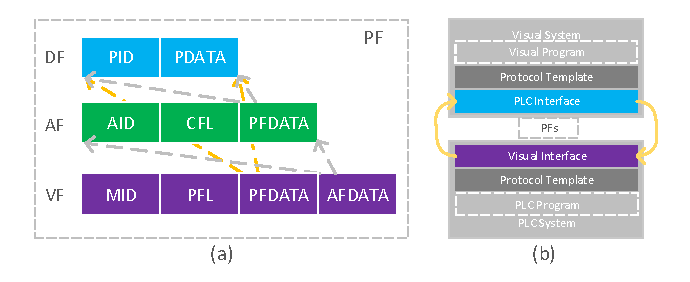
\includegraphics[width=3in]{fig/Protocol.pdf}
		\caption{ (a) The $VCA$ protocol frame contains the parameter and algorithm frames in its data field. The algorithm protocol frame contains several parameter frames. (b) $PF$s interaction between $ePLC$ and $VS$.}
		\label{fig:Protocol}
	\end{figure}
	\subsection{Framing of $PF$}
	The framing contains three steps: $VCA$ framing ($VCAF$), algorithm framing ($AMF$), and parameter framing ($PRF$). The transferring data area ($TD$) saves the data to be transferred, and is indexed by the $PID$. In the $VS$, it represents the parameters obtained from the visual algorithms. In the $ePLC$, the data come from the $RAM$.   
	
	
	\textbf{\emph{VCAF}}: The process is realized as Algorithm \ref{alg1}. It searches for the $PT$ with $mid$ to find the relevant $vlt_x$. We can obtain $man$ and $mdn$ through it. According to $man$ and $mdn$, algorithms \ref{alg3} and \ref{alg2} are called to gain $pfdata$ and $afdata$, respectively. This is then finished after calculating the length ($vfl$).
	
	\textbf{\emph{AMF}}: Algorithm \ref{alg2} illustrates the process and seeks the $PT$ to gain $alt_y$, which contains $apn$. According to $apn$, call Algorithm \ref{alg3} to obtain $pfdata$, then calculate the length ($cfl$) to finish the $AL$ framing.  
	
	\textbf{\emph{PRF}}: Algorithm \ref{alg3} shows the process. The $VS$ obtains $alt_z$ from $FT$, then combines $pid$ and $pdata$.
	
	
	\begin{algorithm}
		\label{alg1}
		\caption{$VCAF$}%算法名字
		%\LinesNumbered %要求显示行号
		\KwIn{$mid$, $TD$}%输入参数
		\KwOut{$PF$}%输出
		SearchPT ($mid$, $vpt_x$)\;
		$PF.mid\leftarrow mid$\; 
		\For{$i=0$;$i<vpt_x.mdn$;$i++$}{
			PRF ($vpt_x$.$cps$[i], $TD$,$pfdata$)\;
		}
		\For{$i=0$;$i<vpt_x.man$;$i++$}{
			AMF ($vpt_x$.$mas$[i], $TD$,$afdata$)\;
		}
		$PF.pfdata\leftarrow$ $pfdata$\; 
		$PF.afdata\leftarrow$ $afdata$\; 
		$PF.vfl\leftarrow$ ($vpt_x.mdn+vpt_x.man$) $\times$ 4 + 8\;
	\end{algorithm}
	
	\begin{algorithm}
		\label{alg2}
		\caption{$AMF$}%算法名字
		%\LinesNumbered %要求显示行号
		\KwIn{$aid$, $TD$, $afdata$}%输入参数
		\KwOut{$afdata$}%输出
		SearchPT ($aid$, $apt_y$)\;
		Create $clf$\;
		$af.aid\leftarrow$ $aid$\;
		\For{$i=0$;$i<apt_y.apn$;$i++$}{
			PRF($apt_y$.$aps$[i], $TD$, $pfdata$)\;
		}
		$af.cfl \leftarrow$ $apt_y.apn \times 4$ + 8\;
		$af.pfdata \leftarrow$ $pfdata$\;	
		$afdata\leftarrow$ $afdata$ + $clf$\;	 
	\end{algorithm}
	\begin{algorithm}
		\label{alg3}
		\caption{$PRF$}%算法名字
		%\LinesNumbered %要求显示行号
		\KwIn{$pid$, $TD$,$pfdata$}%输入参数
		\KwOut{$pfdata$}%输出
		SearchPT ($pid$, $ppt_z$)\;
		Create $pf$\;
		$pf.pid\leftarrow$ $pid$\; %How to address the problem of id is same with address.
		$pf.pdata \leftarrow$ $TD[pid]\times ppt_z.var$\;
		$pfdata\leftarrow$ $pfdata$ + $alf$\;	 
	\end{algorithm}
	
	\subsection{Deframing of $PF$}
	The process of $PF$ deframing is divided into $VCA$ deframing ($VCAD$), $CL$ deframing ($AMD$), and $AL$ deframing ($PRD$). The receiving data ($RD$) area is used to save the deframing parameters. $RD1$, $RD2$, and $RD3$ are the different temporarily stored data area. In $VS$, $RD3$ is the data fed back to the visual algorithms. In the $ePLC$, $RD1$, $RD2$, and $RD3$ denote $LCD$, $MSD$, and $AD$, respectively.
	
	\textbf{\emph{VCAD}}: As illustrated in Algorithm \ref{alg4}, obtain $mid$ and $pfl$ from the starting four and following 4 bytes of data of $PDF$, respectively. Search for $PT$ to gain the relevant $vpt_x$. Send the $pfl-8$ bytes starting from the eighth byte of $PDF+8$ to the address $mda$ of $vlt_x$.
	
	\textbf{\emph{AMD}}: According to $mid$, search for the $PT$ to find the relevant $vpt_x$. Loop deal with the $mda$ times of the parameter frame. In each loop, the data are sent to $RD3$ with the relevant $pid$. Loop deal with the $man$ times of the algorithm frame. In each loop, use $aid$ to find $apt_y$ and send the $afdata$ to the correlative address of $RD2$. Algorithm \ref{alg5} describes the process.
	
	\textbf{\emph{PRD}}: Use $aid$ to obtain its $apt_y$. Loop cope with the algorithm frame $apn$ times. Send the parameters to $RD3$ with the correlative $pid$. Algorithm \ref{alg6} shows the process.
	
	%\begin{figure}
	%	\centering
	%	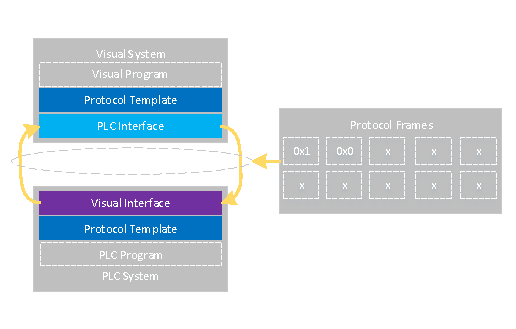
\includegraphics[width=3in]{fig/FlexibleLayer.pdf}
	%	\caption{ $PF$ interaction between PLC interface and visual interface using the agreed communication protocol which is defined as $CID$ in $HPT$ of $PT$. Here, $0x1$ is the $CID$.}
	%	\label{fig:FlexibleLayer}
	%\end{figure}
	\begin{algorithm}
		\label{alg4}
		\caption{$VCAD$}%算法名字
		%\LinesNumbered %要求显示行号
		\KwIn{$PDF$}%输入参数
		$mid \leftarrow$ 4 bytes from $PDF$\;
		searchPT ($mid$, $vpt_x$)\;
		$pfl \leftarrow$ 4 bytes from $PDF+4$\; 
		$RD1[vpt_x.mda]\leftarrow$ $pfl-8$ bytes from $PDF+8$\;     	
		$PDF\leftarrow$ $PDF+pfl$\;
		value of $vpt_x.mdf\leftarrow 1$\;
	\end{algorithm}
	
	\begin{algorithm}
		\label{alg5}
		\caption{$AMD$}%算法名字
		%\LinesNumbered %要求显示行号
		\KwIn{$mid$}%输入参数
		searchPT($mid$, $vpt_x$)\;
		$mda\leftarrow$ $vpt_x.mda$\;	
		\For{$i=0$;$i<vpt_x.mdn$;$i++$}{
			$RD3[RD1[mda]]\leftarrow$ 4 bytes from $mda+4$\;
			$mda\leftarrow mda+8$\;
		}
		\For{$i=0$;$i<vpt_x.man$;$i++$}{
			searchPT($vpt_x.mas[i]$, $apt_y$)\;
			$cfl\leftarrow$ 4 bytes from $mda+4$\;
			$RD2[apt_y.apa]\leftarrow$ $cfl - 8$ bytes from $mda+8$\; 
			$mda\leftarrow$ $mda+cfl$\;
			value of $apt_y.adf\leftarrow$ 1\; 
		}
	\end{algorithm}
	
	\begin{algorithm}
		\label{alg6}
		\caption{$PRD$}%算法名字
		%\LinesNumbered %要求显示行号
		\KwIn{$aid$}%输入参数
		searchPT($aid$, $apt_y$)\;
		$ada\leftarrow$ $apt_y.ada$\;
		\For{$i=0$;$i<apt_y.apn$;$i++$}{
			$RD3[RD2[ada]]\leftarrow$ 4 bytes from $ada+4$\;
			$ada\leftarrow ada+8$\;
		}
	\end{algorithm}
	\subsection{Process of the Algorithms}
	
	The execution sequence of the six algorithms is $PRF$, $AMF$, $VCAF$, $VCAD$, $AMD$, and $PRD$. $VCAF$ will particularly call the $PRF$ to frame the control relevant parameters. The direction of transfer $PF$s could be from $VS$ to $ePLC$ or from $ePLC$ to $VS$. From $VS$ to $ePLC$, $PRF$, $AMF$, and $VCAF$ are running in $VS$, and the remaining algorithms are running in $ePLC$. From $ePLC$ to $VS$, $PRF$, $AMF$, and $VCAF$ are running in $ePLC$, and the remaining algorithms are running in $VS$.
	%
	%\begin{figure}
	%	\centering
	%	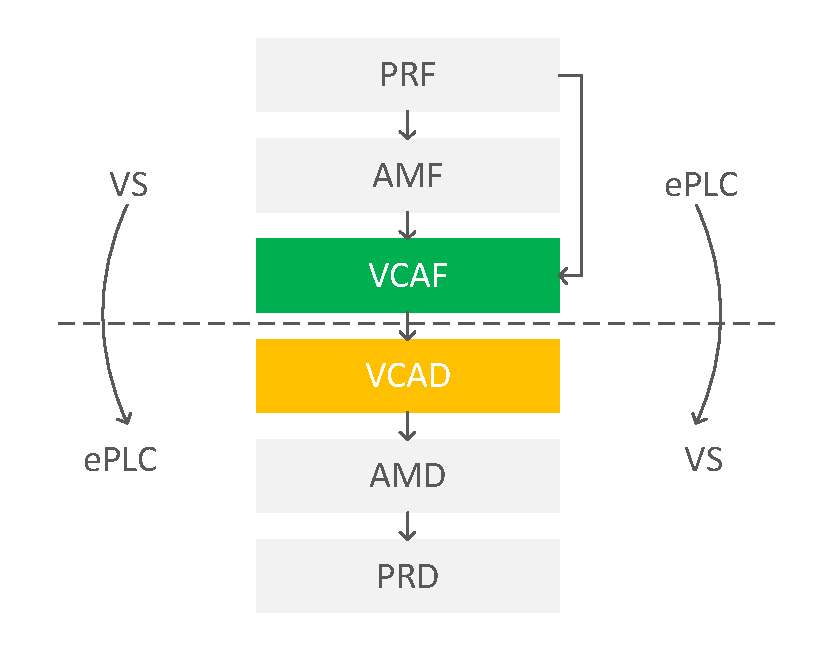
\includegraphics[width=3in]{fig/Algorithms.pdf}
	%	\caption{ Process of the six algorithms and the execution sequence is $PRF$, $AMF$, $VCAF$, $VCAD$, $AMD$, and $PRD$; and the $VCAF$ will particularly call the $PRF$ to frame the control relevant parameters. The direction of transfer $PF$s could be form $VS$ to $ePLC$ or form $ePLC$ to $VS$.}
	%	\label{fig:Algorithms}
	%\end{figure}
	
	\section{System Operation Mechanism}
	\label{Execution}
	\subsection{Implementation of Flexible Program and Execution}
	$FL$ contains the PLC interface and the visual interface shown in Fig. \ref{fig:Protocol} (b).
	%Fig. \ref{fig:FlexibleLayer}. 
	They interact with each other using the agreed communication protocol defined as the $CID$ in the $HPT$ of the $PT$. 
	
	In the $ePLC$, the visual interface includes the following parts:
	
	\textbf{V1}: communicates with the $VS$ according to the $CID$ in the $HPT$, and has three transitions: \textbf{V1.1} denotes no communication and other operations; \textbf{V1.2} denotes receiving $PF$s from the $VS$; and \textbf{V1.3} denotes sending $PF$s to the $VS$. In $V1.3$, the $PF$s will be saved in the $VD$ of the $ePLC$, and two pointers are found, $PDF$ and $PSP$ (Fig. \ref{fig:VisualInterface}). The $PDF$ points to the address of deframing $PF$, while the $PSP$ points to the address of saving $PF$. After saving the $PF$, the $PSP$ will point to the next new address according to the $vfl$ of the $PF$. In $V1.3$, the visual interface frames the $TD$ into the $PF$ with algorithms \ref{alg1}, \ref{alg2} and \ref{alg3}. Here, the $TD$ is in the $RAM$ of the $ePLC$.
	
	\textbf{V2}: Algorithm \ref{alg4} will be called. The $PDF$ will point to the next $PF$ if a $PF$ is deframed.
	
	
	The following parts are in the $VS$:
	
	\textbf{V3}: visual algorithms extract the useful data and stores them into the array of data required to be transferred ($TD$), in which the parameters could be indexed by the $PID$.
	
	\textbf{V4}: communicates with the $ePLC$ and contains three transitions: \textbf{V4.1} has no communication and other operations; \textbf{V4.2} frames the $TD$ into the $PF$s with algorithms \ref{alg1}, \ref{alg2}, and \ref{alg3} and sends the $PF$s to the $ePLC$ (here, the $TD$ is an array in the $VS$); and \textbf{V4.3} receives the $PF$s from the $ePLC$ and deframes the $PF$s with algorithms \ref{alg4}, \ref{alg5}, and \ref{alg6}.
	
	\begin{figure}
		\centering
		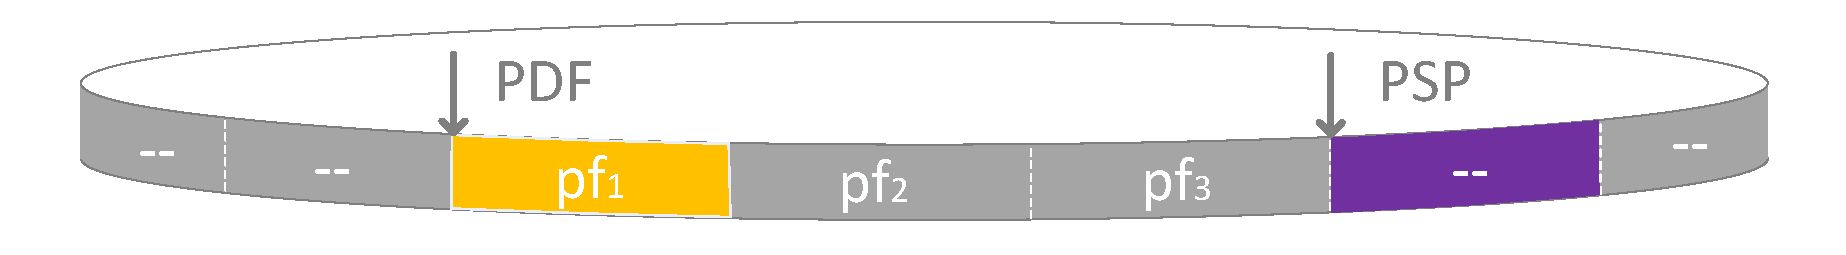
\includegraphics[width=3in]{fig/VisualInterface.pdf}
		\caption{ Process of $PDF$ and $PSP$. 
			%		$PDF$ points to the address of deframing $PF$ and $PSP$ points to the address of saving $PF$. The $PDF$ will point to the next address of $PF$ if a $PF$ is deframed. After saved the $PF$, the $PSP$ will point to the next new address according the $vfl$ of $PF$.
		}
		\label{fig:VisualInterface}
	\end{figure}
	
	
	
	\subsection{Implementation of the Control Program and Execution}
	The control program ($CP$) is responsible for organizing the modules, executing the logic program, deframing the $PF$, and handling data interaction with the algorithm program. The implementation of the control program is described below:
	
	\textbf{C1}: traverses the $MCF$ and the $MDF$ and contains three transitions: \textbf{C1.1} means that every $mcf\in MCF$ and $mdf \in MDF$ is recovered to zero; \textbf{C1.2} means that both $mcf_i$ and $mdf_i$ are checked as one; and \textbf{C1.3} means that $mcf_i$ is checked as one, while $mdf_i$ is zero.
	
	\textbf{C2}: executes Algorithm \ref{alg5}. 
	
	\textbf{C3}: executes the logic program and checks whether there are any data required to transfer.  
	
	\textbf{C4}: $\mathcal{P}_{mts}$ is used to send data and inform the slave processor to receive parameters and start algorithms.   
	
	\textbf{C5}: checks the end of this module. \textbf{C5.1} states that this module executes once. \textbf{C5.2} states that the logic program is still required to run.  
	
	\subsection{Implementation and Execution of the Algorithm Program }
	The algorithm program ($AP$) is in $EL$. $AP=\{\mathcal{P}_{stm}, AS, ALDP\}$, where $\mathcal{P}_{stm}$ feeds back data to the master processor; $AS$ contains all algorithms; and $ALDP$ deframes the $AL$ frame. The execution of the algorithm program is introduced below:
	
	\textbf{A1}: traverses $AFS$, $ADF$, and $SMB$. \textbf{A1.1} is not a program required to execute. \textbf{A1.2} denotes that $PF$s that needed to be deframed are checked. \textbf{A1.3} denotes that data need to be fed back to the master processor. \textbf{A1.4} denotes that an algorithm that needs to be executed is checked. \textbf{A1.5} denotes that the parameters of an algorithm that needed to be updated are checked.  
	
	\textbf{A2}: $ALDP$ is executed to call Algorithm \ref{alg5}. 
	
	\textbf{A3}: the $\mathcal{P}_{stm}$ is used to feed data back to the master processor. 
	
	\textbf{A4}: starts an algorithm.
	
	\textbf{A5}: executes the algorithm until the end. 
	
	\subsection{Petri-Net-based Execution of Threads}
	We adopt the analogous thread structure in \cite{wu2018customized}. Three special threads are illustrated: 1) the visual thread is responsible for the interaction with $VS$ and drives the flexible layer; 2) the control thread is mainly responsible for organizing the whole program and driving the control layer; and 3) the algorithm thread is used to drive the algorithm layer.
	
	\begin{figure}
		\centering
		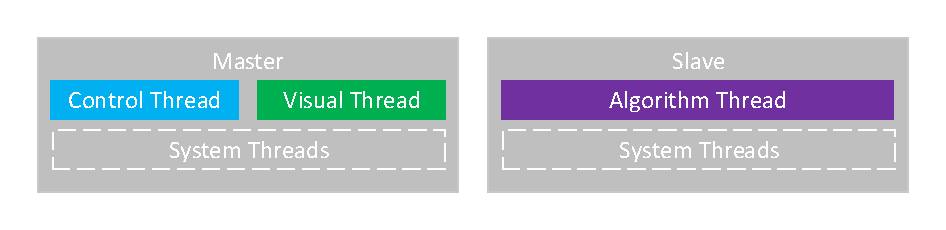
\includegraphics[width=3in]{fig/Threads.pdf}
		\caption{ Thread structure with three special threads: visual, control, and algorithm threads. The control and visual threads run in the master slave, while the algorithm thread runs in the slave thread.}
		\label{fig:Threads}
	\end{figure}
	
	In our works, Petri Net is adopted to describe the execution of the three threads. Every thread is a Petri-Net, and we define the Petri Net as a three tuple:
	
	\begin{equation}
	PN = \{P,T,F\},
	\end{equation} 
	where $P$ is the finite set of places; $T$ is the finite set of transitions; and $F$ is the set of arcs. $F \subset P\times T \cup T\times P$ denotes that the arcs are from $P$ to $T$ and from $T$ to $P$.
	
	We can then define the execution of threads ($ET$) as follows:
	\begin{equation}
	ET = \{PN_V,PN_C,PN_A\},
	\end{equation} 
	where $PN_V,PN_C,PN_A$ are the Petri Net of the visual, control, and algorithm threads, respectively. $ET$ is described in Fig. \ref{fig:threadExecution}.
	
	$PN_V$ is presented as follows:
	\begin{equation}
	\left\{
	\begin{array}{l}
	PN_V= \{P_V,T_V,F_V\},\\
	P_V=\{P_{V1}, P_{V2}, P_{V3}\},\\
	T_V=\{V_1,V_2\},\\
	\end{array}
	\right.
	\end{equation} 
	where $P_{V1}$ is idle; $P_{V2}$ is $PDF != PSP$; and $P_{V3}$ denotes that a relevant $mdf$ is set.
	
	$PN_C$ is denoted as follows:
	\begin{equation}
	\left\{
	\begin{array}{l}
	PN_C= \{P_C,T_C,F_C\},\\
	P_C=\{P_{C1}, P_{C2}, P_{C3}, P_{C4}, P_{C5}, P_{C6}\},\\
	T_C=\{C_1,C_2,C_3,C_4,C_5\},\\
	\end{array}
	\right.
	\end{equation} 
	where $P_{C1}$ is idle; $P_{C2}$ denotes that a model is started, and $mdf_i$ is one; $P_{C3}$ denotes that a model is started, and $mdf_i$ is zero; $P_{C4}$ denotes that any $msb_i$ is one; $P_{C5}$ means the end of the data interaction, in which the  correlative $msf$ is zero; and $P_{C6}$ denotes that a module finishes a one-time execution.
	
	$PN_V$ is illustrated as follows:
	\begin{equation}
	\left\{
	\begin{array}{l}
	PN_A= \{P_A,T_A,F_A\},\\
	P_A=\{P_{A1}, P_{A2}, P_{A3}, P_{A4}, P_{A5}, P_{A6}, P_{A7}, P_{A8}\},\\
	T_A=\{A_1,A_2,A_3,A_4,A_5\},\\
	\end{array}
	\right.
	\end{equation} 
	where $P_{A1}$ is idle; $P_{A2}$ denotes that $adf_i$ is one; $P_{A3}$ denotes that any $adf_i$ is zero; $P_{A4}$ denotes that $smb_i$ is one; $P_{A5}$ denotes that any $smf_i$ is zero; $P_{A6}$ denotes that $afe_i$ is one; $P_{A7}$ presents that $afs_i$ is one; and $P_{A8}$ denotes that any $afe_i$ is zero.   
	
	%The $ET$ is described in Fig. \ref{fig:threadExecution}. In the Petri Net of visual thread, if $V1.2$ executes and receives a $PF$ from $VS$, it transits from the initial position of $P_{V1}$ to $P_{v2}$. After finished deframing of a $PF$, the state transits to $P_{V3}$ and then visual thread back to execute $V1$. If there is any $FS$ which should be sent to $VS$, it will execute $V1.2$. Apart from that, it will execute $V1.1$ and back to the position of $P_{V1}$.
	%
	%In the Petri Net of control thread, the control thread executes the $C1$. The difference between $P_{C1.2}$ and $P_{C1.3}$ is that after $P_{1.2}$, the control thread transits to $P_{C2}$ and executes $C2$. Except that, it will back to $P_{C1}$. Then, the control thread runs into a module and $C3$ is run. If find any data needed to transfer to slave processor, it transits to $P_{C4}$ and executes $C4$. When finish transfer, it transits to $P_{C5}$. After execution of $C5$, according to $C5.1$ and $C5.2$, control thread transits to $P_{C3}$ and $P_{C6}$. The previous one is executed owing to that the logic program of this module is not finished.
	%
	%In the Petri Net of algorithm thread, the $A1$ is executed; if any $AF$ needed to deframe, algorithm thread transits to $P_{A2}$ and after the execution of $A2$, it transits to $P_{A2}$; if any data required to feed back to master processor, algorithm thread transits to $P_{A4}$, then transfers the data, and transits to $P_{A5}$; if any algorithm should be started, algorithm thread transits to $P_{A6}$, executes the $A4$, transits to $P_{A7}$, executes $A5$ to update the parameters, and then transits to $P_{A8}$; if there are algorithms running and needed to updates parameters, algorithm thread transits to $P_{A7}$ directly and after the execution of $A5$ transits to $P_{A8}$; and above-mentioned transitions of $V1$ are executed in sequence.               
	
	\begin{figure}
		\centering
		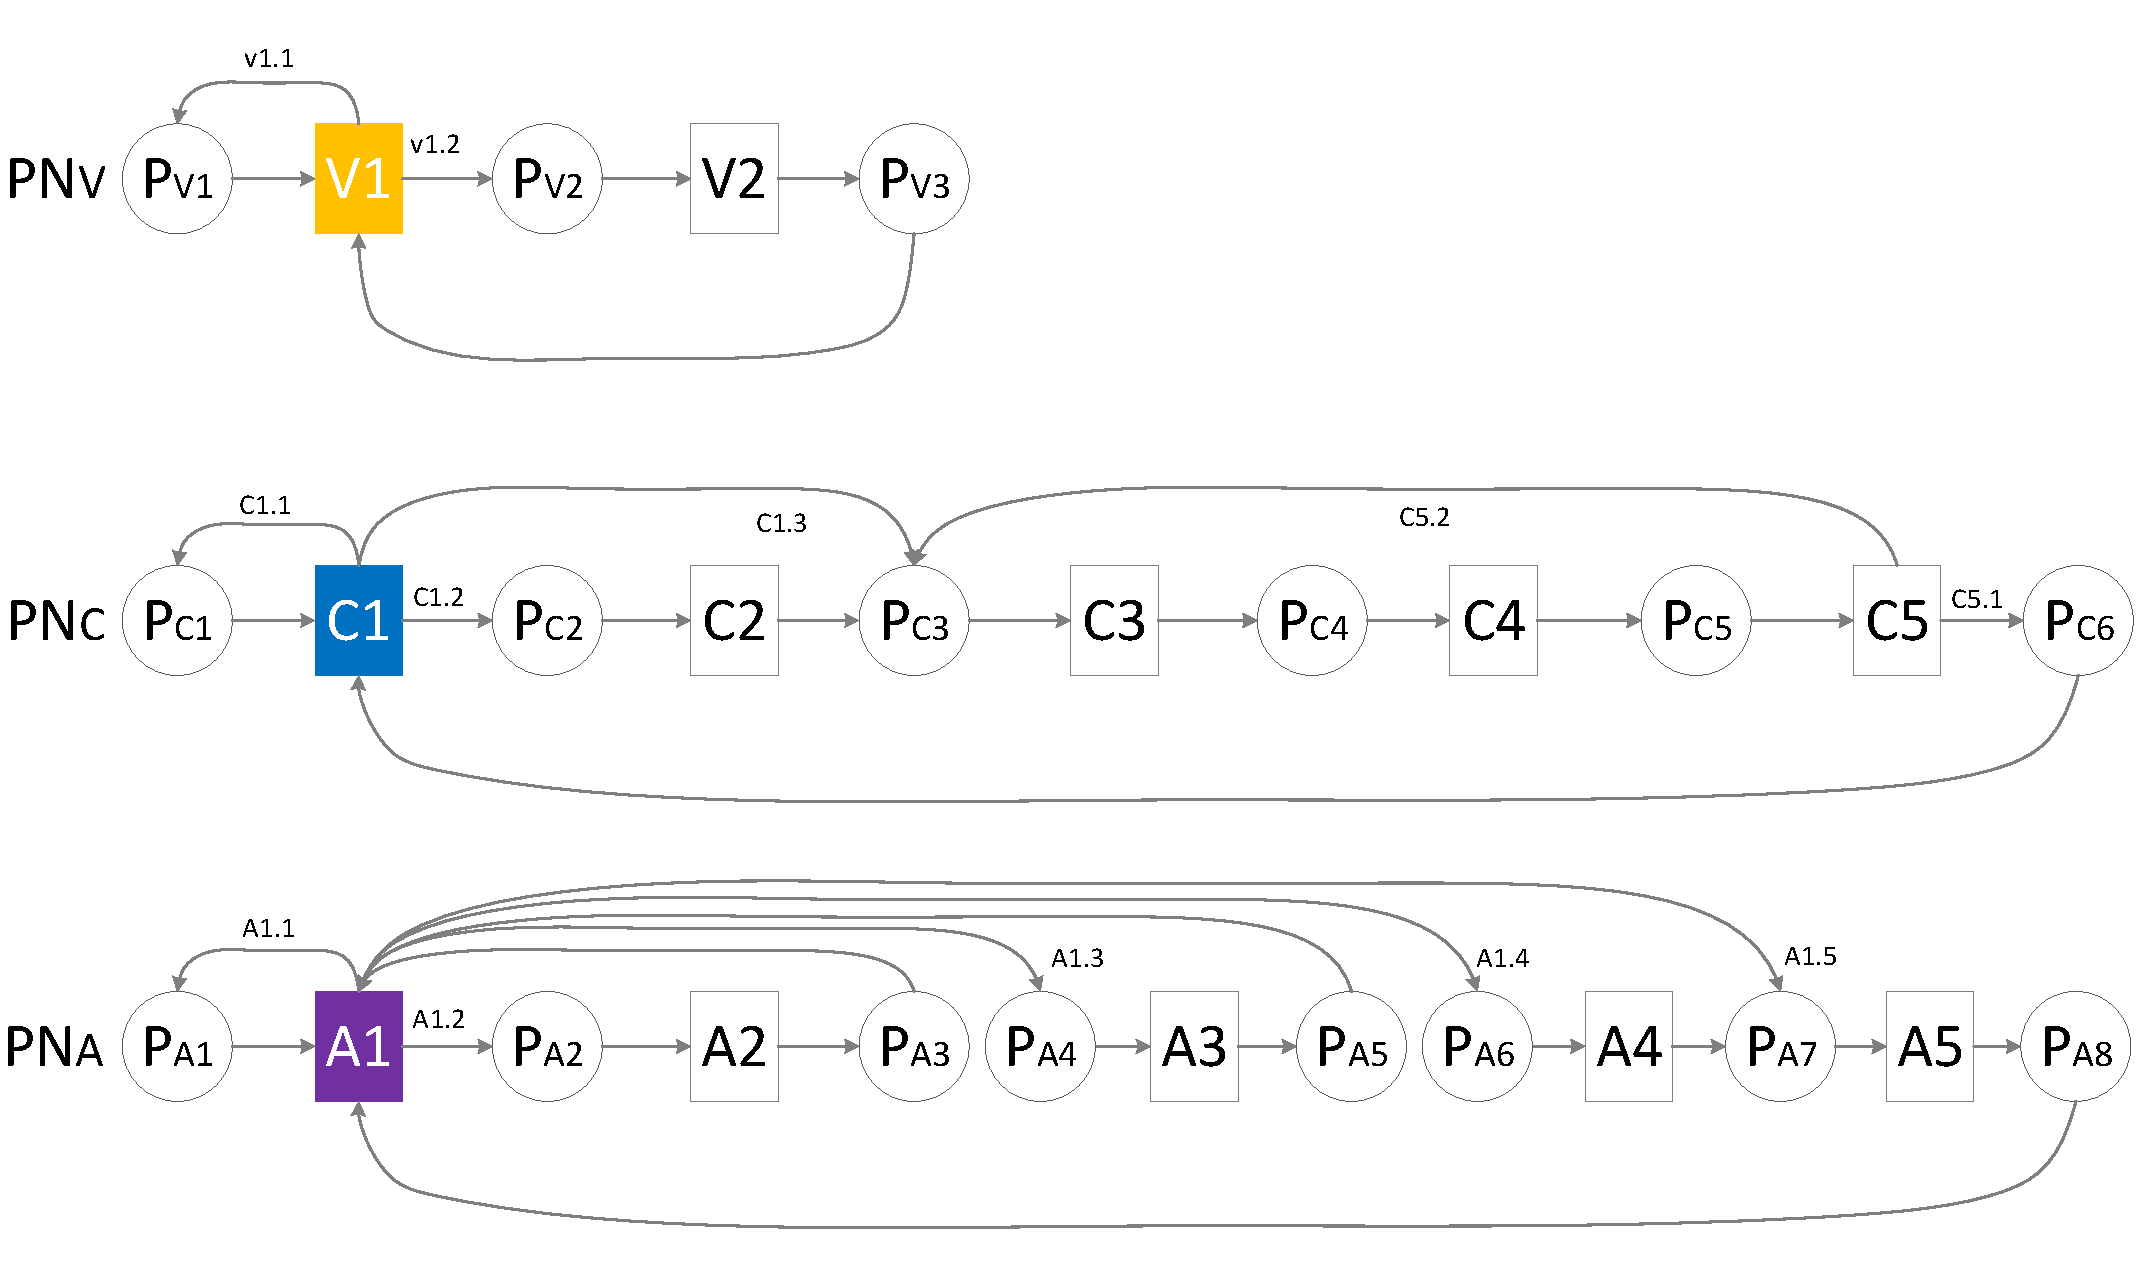
\includegraphics[width=3in]{fig/ThreadExecution.pdf}
		\caption{ Process of $ET$ and its contained Petri Nets of the visual, control, and algorithm threads.}
		\label{fig:threadExecution}
	\end{figure}
	
	\section{Case Analysis}
	\label{Case}
	This section introduces two scenarios of the proposed $VCA$ protocol-based integration method in $ePLC$. With the $VCA$ protocol, the users only need to code additional algorithms and change the $PT$ when the scenario of the visual servo system is changed. 
	
	\subsection{Case one: Winding Machine with a Visual System}
	
	As shown in Fig. \ref{fig:Winding}, 
	(a) is the visual system, whose processor is the ARM9-based S3C2440 and uses the CAN interface to communicate with the OV9650 CMOS camera; (b) is the $ePLC$, CASS-PLCA149B; (c) is the winding machine with a visual system that contains two axes: the U-axis and the Q-axis; (d) shows the winding effect; and (e) shows the angle of $\theta$, Q-axis, and U-axis.
	In the winding process, the tension of the copper wire will irregularly change, especially for the thick ones. However, we used the same speed ratio of the U-axis and the Q-axis, which always leads to the irregularity of each coil layer. Hence, we can use the visual system to decrease or increase the speed of the Q-axis to control the wire angle. 
	
	%Figure \ref{fig:WindingSystem} is 
	In the structure of the winding machine system, the ePLC has two chips: a master chip and a slave chip. It uses RS232 to receive $PF$s, and could control six servo systems at most. The winding machine has two axes: the U-axis and the Q-axis. $VS$ uses the CMOS camera to gain winding images and transfer the digital information to the ARM CUP. The ARM CUP will extract parameters from the digital information, frame $PF$s, and transfer $PF$s to $ePLC$ continuously. 
	
	
	\subsubsection{Design of $PT$}
	In \cite{wu2018customized}, we propose the customized winding machine language, which only contains 13 instructions. Here, we can use the second and third instructions to control the U-axis and the Q-axis, respectively. In the algorithm layer, both use the same motion control algorithm, which controls one axis with speed and position. The winding process mainly aims to control the speed ratio of the U-axis and the Q-axis; hence, we use the $VS$ to influence the speed of the Q-axis only. Table \ref{table:PTofWinding} presents the $PT$ of the winding machine, in which $pid_1$ is the speed of the Q-axis, and 1000 of $var_1$ is used to multiply by $\theta$.
	\begin{table}
		\scriptsize \caption{$PT$ of winding machine}
		\label{table:PTofWinding}
		\begin{threeparttable}
			\renewcommand{\arraystretch}{1.4}
			\setlength\tabcolsep{3pt}
			\begin{tabular}{|p{1cm}|p{1cm}|p{1cm}|p{1cm}|p{1cm}|p{1cm}|p{1cm}|}
				\hline
				$cid_1$: & $tda_1:$   &- &-& -  &- &- \\
				0x01\tnote{*}&0x00&& &&&\\
				\hline
				$mid_1$:   & $man_1$: &$mdn_1$: &$mda_1$:&$msf_1$:& $mdf_1$:  & $mas_1$:\\
				0x01      & 1     &   0    &0X200   &0X400   & 0X600  &0x01 \\
				\hline
				$aid_1$:  & $apn_1$:& $af_1$: &$ada_1$: &$aps1_1$:  &-&-\\
				0x01     & 0X1    & 0X14A  &0x400 &0X0   & &\\
				\hline
				$pid_1$:  &$vid_1$: &$var_1$: &-  &-  &- &-\\
				0X0      & 0X1    & 0x200   &         &   & &\\
		    	\hline
			\end{tabular}
			\begin{tablenotes}
				\footnotesize
				\item[*] This number is hexadecimal, and the item means that the value of $cid_1$ is 0x01.
			\end{tablenotes}
		\end{threeparttable}
	\end{table}
	\subsubsection{Process of $PF$}
	Table \ref{table:PFofWinding} shows the interacted $PF$ between $VS$ and $ePLC$. First, $VS$ detects that $\theta$ is 2 degrees. It then sends the $PF$ to inform the $ePLC$ to increase the Q-axis speed of 2000 pulses per millisecond (p/ms). The increment of the Q-axis speed is changed to 1000 p/ms when the $\theta$ decreases to 1 degree. The $\theta$ has recovered to 0; hence, the $ePLC$ is informed to recover the initial speed of the Q-axis.  
	\begin{table}
		\scriptsize \caption{$PF$ of winding machine}
		\label{table:PFofWinding}
		\begin{center}
			\renewcommand{\arraystretch}{1.4}
			\setlength\tabcolsep{3pt}
			\begin{tabular}{|p{1.2cm}|p{1.2cm}|p{1.2cm}|p{1.2cm}|p{1.2cm}|p{1cm}|}
				\hline
				$mid_1$  & $pfl_1$ &$aid_1$ & $cfl_1$  & $pid_1$  &$pdata_1$   \\
				\hline
				0x01    & 0x14  &0x01  &0xE     &0x01   &0x400   \\
				\hline
				0x01    & 0x14  &0x01  &0xE     &0x01   &0x200   \\
				\hline
				0x01    & 0x14  &0x01  &0xE     &0x01   &0x000   \\
				\hline
			\end{tabular}
		\end{center}
	\end{table}
	\begin{figure}
		\centering
		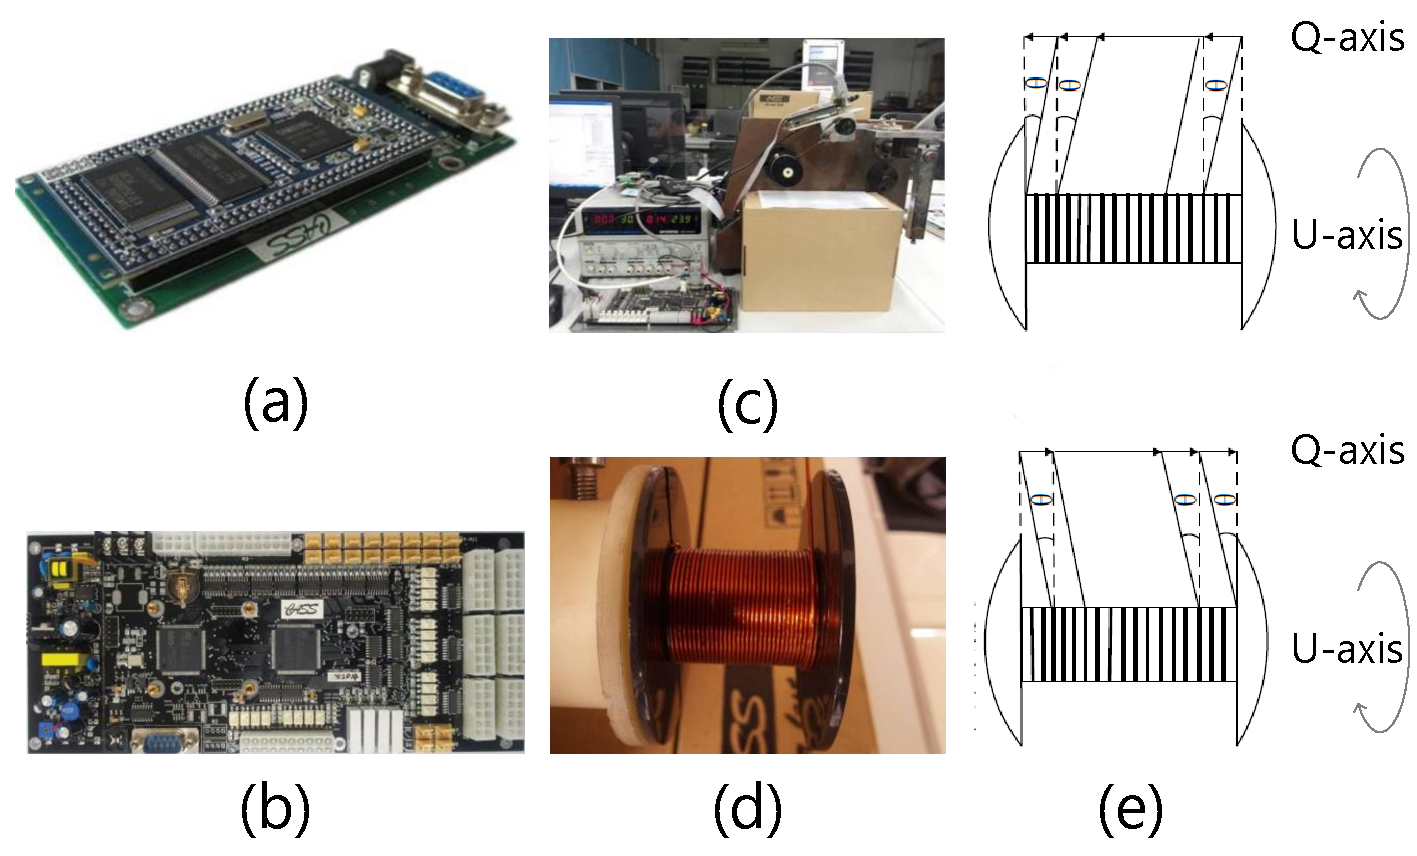
\includegraphics[width=3in]{fig/Winding.pdf}
		\caption{(a) is the visual system, whose processor is the ARM9-based S3C2440 and uses the CAN interface to communicate with the OV9650 CMOS camera; (b) is the $ePLC$, CASS-PLCA149B; (c) is the winding machine with a visual system that contains two axes: the U-axis and the Q-axis; (d) shows the winding effect; and (e) shows the angle of $\theta$, Q-axis, and U-axis.
		}
		\label{fig:Winding}
	\end{figure}
	%\begin{figure}
	%	\centering
	%	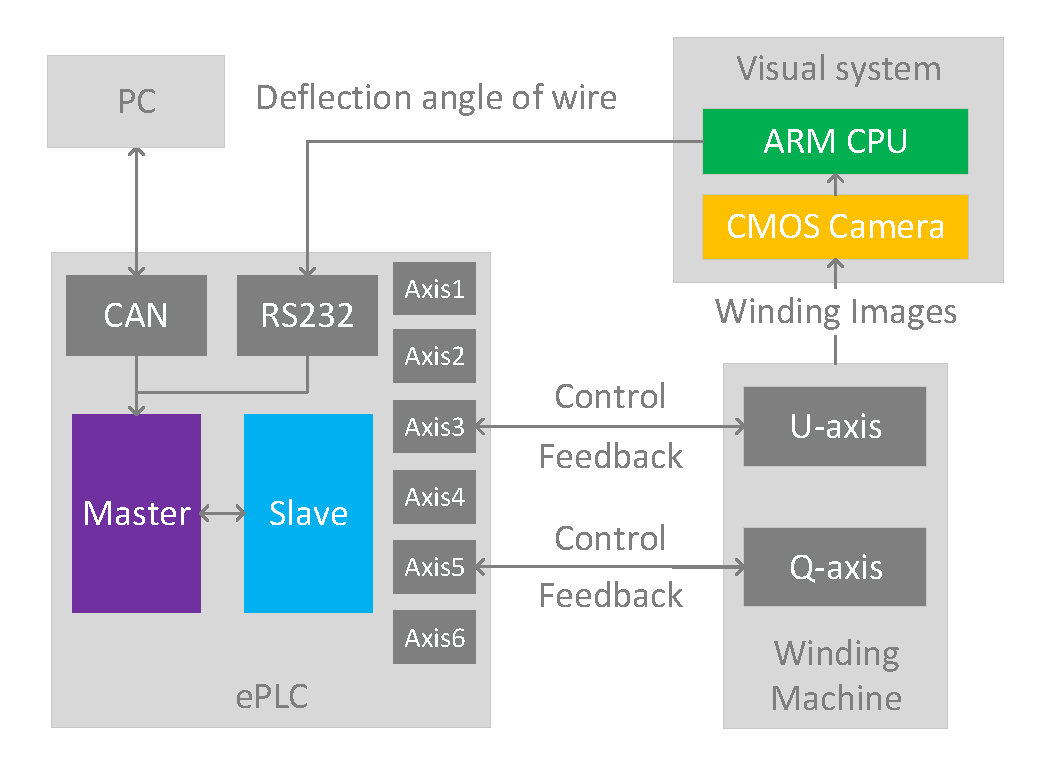
\includegraphics[width=3in]{fig/WindingSystem.pdf}
	%	\caption{ Structure of the winding machine system. The ePLC has two chips: a master chip and a slave chip. It uses the RS232 to receive $PF$s and could control six servo systems at most. The winding machine has two axes: The U-axis and Q-axis. The $VS$ use the CMOS camera to gain winding images and transfer the digital information to ARM CUP. The ARM CUP will extract parameters, frame $PF$s and transfer them to $ePLC$ continuously.}
	%	\label{fig:WindingSystem}
	%\end{figure}
	
	\subsection{Results of Case One}
	The advantages from case one indicate that:
	1) The software architecture is clearly divided into the flexible, control, and algorithm layers. The same control program and algorithms could be reused. The separated control and algorithm layer programs could be developed by different-level programmers when a new application has some customized requirements.
	2) The parameters that interacted between the $VS$ and the $ePLC$ could be associated using the $PT$. Meanwhile, the $PF$s contained the parameters that could be carried to every layer. Hence, when more parameters need to be interacted, only the $PT$ should be changed without reprogramming.
	3) The customized structure of the $ePLC$, favorable memory allocation, and Petri-Net-based multi-threading structure make it possible for high-performance algorithms to run in a single processor. From the view of applications, the proposed architecture can also be easily applied to very different cases.
	
	
	\subsection{Case Two: Binocular Catching Robot}
	\begin{figure}
		\centering
		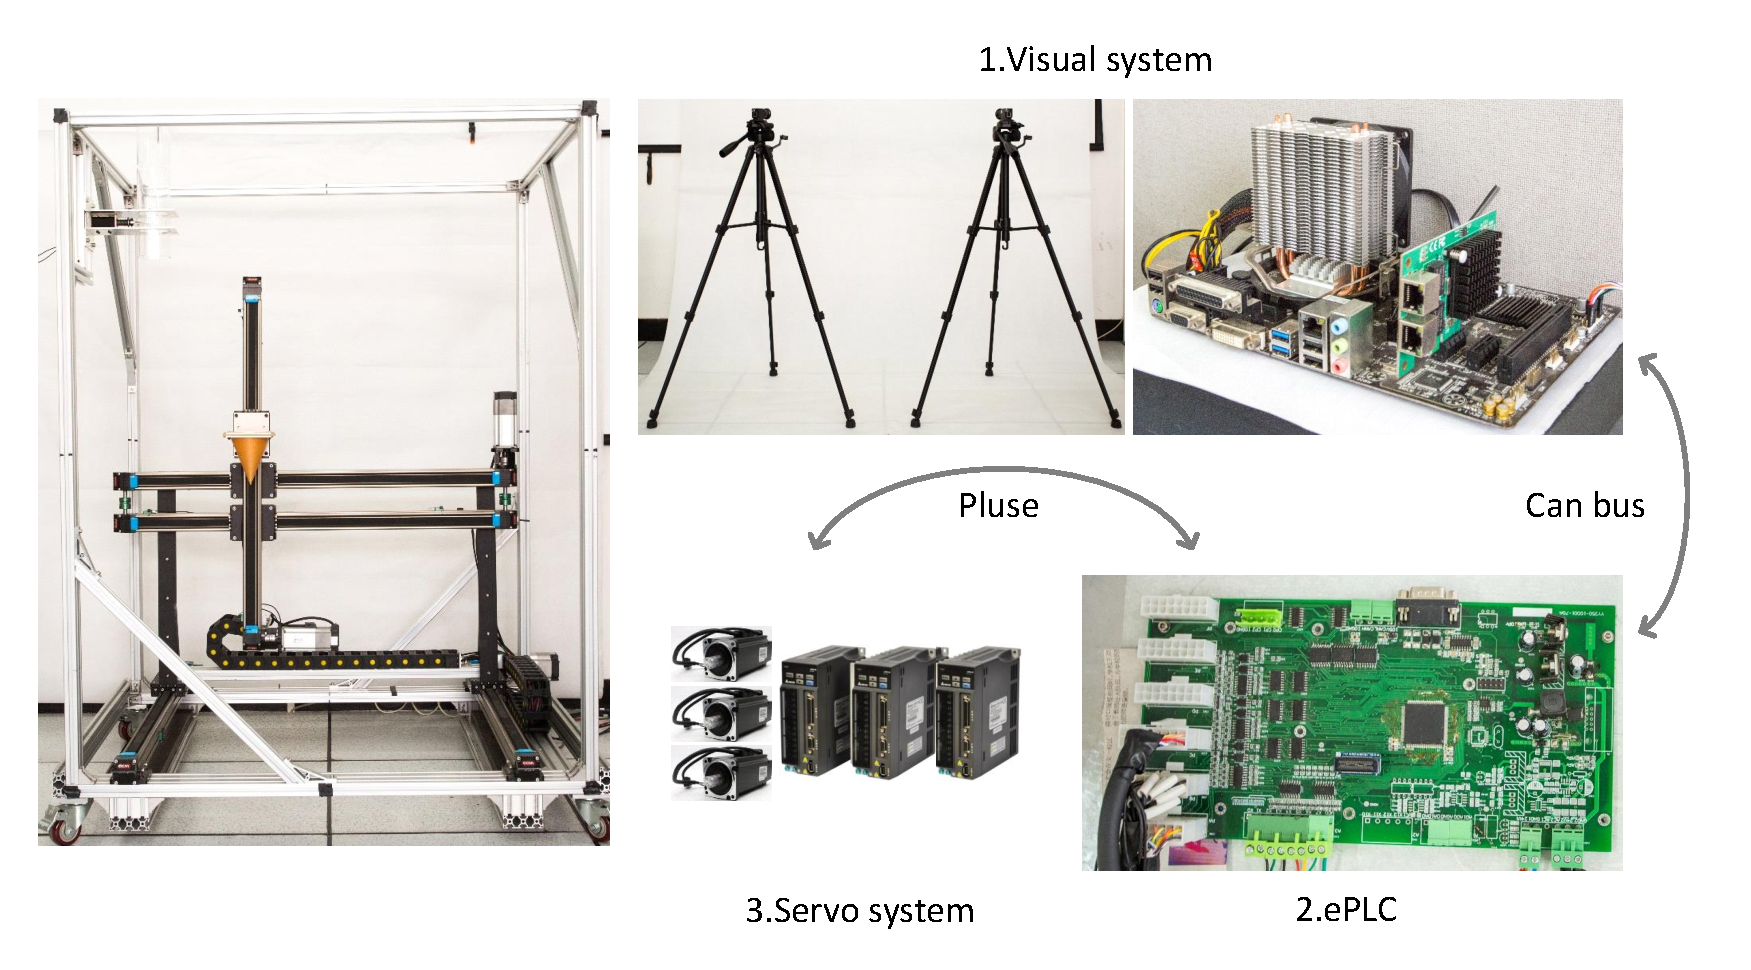
\includegraphics[width=3in]{fig/robot.pdf}
		\caption{ The binocular catching robot consists of the visual system, $ePLC$, and servo system.}
		\label{fig:robot}
	\end{figure}
	Fig. \ref{fig:robot} shows that the binocular catching robot adopts two cameras to judge the ball position in the space. By continuously sending parameters to the $ePLC$, the robot runs to the position to catch the ball and finally catches it. The cameras and the lens used are GE31GC and FA0401C, respectively. The visual system is GIGABYTE's GA-B85M-D3V-A. The $ePLC$ uses a TI F28M35 chip with two cores, namely ARM Cortex M3 and TI C28x, which contain a shared RAM. The adopted servo system is ASDA-B2. 
	\subsubsection{Design of $PT$}
	The $ePLC$ is designed to control six parallel axes. We adopt the same algorithm of the Q-axis and the U-axis in case one, while we name the three axes of the Cartesian robot as the X-axis, Y-axis, and Z-axis. In this case, we have the similar module with case one, but it contains three motion algorithms. $pid_1$ and $pid_2$ are the position and the speed of the X-axis, respectively. $pid_3$ and $pid_4$ are the position and the speed of the Y-axis, respectively. $pid_5$ and $pid_6$ are the position and the speed of the Z-axis, respectively. The $VS$ uses meter and meter per second (m/s) to measure the distance and the speed, respectively. Meanwhile, in the $ePLC$, driving every 1 mm needs to output 100 pluses. Hence, the $VAR$ of the position and the speed are both 100. 
	\begin{table}
		\scriptsize \caption{$PT$ of binocular catching robot}
		\label{table:PTofRobot}
		\begin{center}
			\renewcommand{\arraystretch}{1.4}
			\setlength\tabcolsep{3pt}
			\begin{tabular}{|c|c|c|c|c|c|c|c|c|}
				\hline
				$cid_1$:  & $tda_1$:   &- &-& -  &- &-&-&- \\
				0x01&0x00&& &&&&&\\
				\hline
				$mid_1$:&$man_1$:&$mdn_1$:&$mda_1$:&$msf_1$:&$mdf_1$:&$mas_1$:&$mas_1$:&$mas_1$:\\
				0x01  &0x1 &   0    &0X200  &0X400  & 0X600 &0x01   &0x02   &0x03 \\
				\hline
				$aid_1$:  & $apn_1$:& $af_1$: &$ada_1$: &$aps1_1$:  &$aps2_1$:&-&-&-\\
				0x01     & 0X2    & 0X14A  &0x400 &0X0   &0x4 &&&\\
				\hline
				$aid_2$:  & $apn_2$:& $af_2$: &$ada_2$: &$aps1_2$:  &$aps2_2$:&-&-&-\\
				0x02     & 0X2    & 0X14B  &0x410  &0X8       &0xA &&&\\
				\hline
				$aid_3$:&$apn_3$:&$af_3$:&$ada_3$:&$aps1_3$:&$aps2_3$:&-&-&-\\
				0x03     & 0X2    & 0X14C  &0x420   &0XE       &0X10 &&&\\
				\hline
				$pid_1$:&$vid_1$:&$var_1$:&$pid_2$:&$vid_2$:&$var_2$: &$pid_3$:&$vid_3$:&$var_3$:\\
				0X0      & 0X1    & 0x40  &0X4     &0X1    & 0x40  &0X8      & 0X1    & 0x40\\
				\hline
				$pid_4$  &$vid_4$ &$var_4$ &$pid_5$ &$vid_5$&$var_5$ &$pid_6$  &$vid_6$ &$var_6$\\
				\hline
				0XA      & 0X1    & 0x40  &0XE     &0X1    & 0x40  &0X10     & 0X1    & 0x40\\
				\hline
			\end{tabular}
		\end{center}
	\end{table}
	
	
	\begin{table*}
		\scriptsize \caption{$PF$ of binocular catching robot}
		\label{table:PFofrobot}
		\begin{center}
			\renewcommand{\arraystretch}{1.4}
			\setlength\tabcolsep{3pt}
			\begin{tabular}{|c|c|c|c|c|c|c|c|c|c|c|c|c|c|c|c|c|c|c|c|}
				\hline
				$mid_1$   & $pfl_1$ 
				&$aid_1$  & $cfl_1$  & $pid_1$  &$pdata_1$ & $pid_2$  &$pdata_2$
				&$aid_2$  & $cfl_2$  & $pid_3$  &$pdata_3$ & $pid_4$  &$pdata_4$
				&$aid_3$  & $cfl_3$  & $pid_5$  &$pdata_5$ & $pid_6$  &$pdata_6$  \\
				\hline
				0x01    & 0x14  
				&0x01  &0xE     &0x00   &0x1C6   &0x04   &0x10A5E 
				&0x02  &0xE     &0x08   &0x17b   &0x0A   &0xDE27
				&0x03  &0xE     &0x0E   &0x140   &0x10   &0xBB80\\
				\hline
				0x01    & 0x14  
				&0x01  &0xE     &0x00   &0x1F6   &0x04   &0x126AA 
				&0x03  &0xE     &0x08   &0x175   &0x0A   &0xDA94
				&0x04  &0xE     &0x0E   &0x140   &0x10   &0xBB80\\	
				\hline
				0x01    & 0x14  
				&0x01  &0xE     &0x00   &0x28F   &0x04   &0x17FDB 
				&0x02  &0xE     &0x08   &0x17A   &0x0A   &0xE0D8
				&0x03  &0xE     &0x0E   &0x140   &0x10   &0xBB80\\
				\hline
				0x01    & 0x14  
				&0x01  &0xE     &0x00   &0x263   &0x04   &0x16624
				&0x02  &0xE     &0x08   &0x171   &0x0A   &0xD87D
				&0x03  &0xE     &0x0E   &0x140   &0x10   &0xBB80\\		
				\hline
			\end{tabular}
		\end{center}
	\end{table*}
	\subsubsection{Process of $PF$}
	Table \ref{table:PFofrobot} shows the $PF$s of the time spent catching the ball. Fig. \ref{fig:Trajectory} depicts the ball trajectory, which is the trajectory captured by the cameras. The red point denotes the position where the ball is thrown. The blue points are the positions where the catching points are predicted. The yellow points are the predictive catch points. The $VS$ sends the $PF$ to $ePLC$ to adjust the destination and the speed of every axis.
	
	\begin{figure}
		\centering
		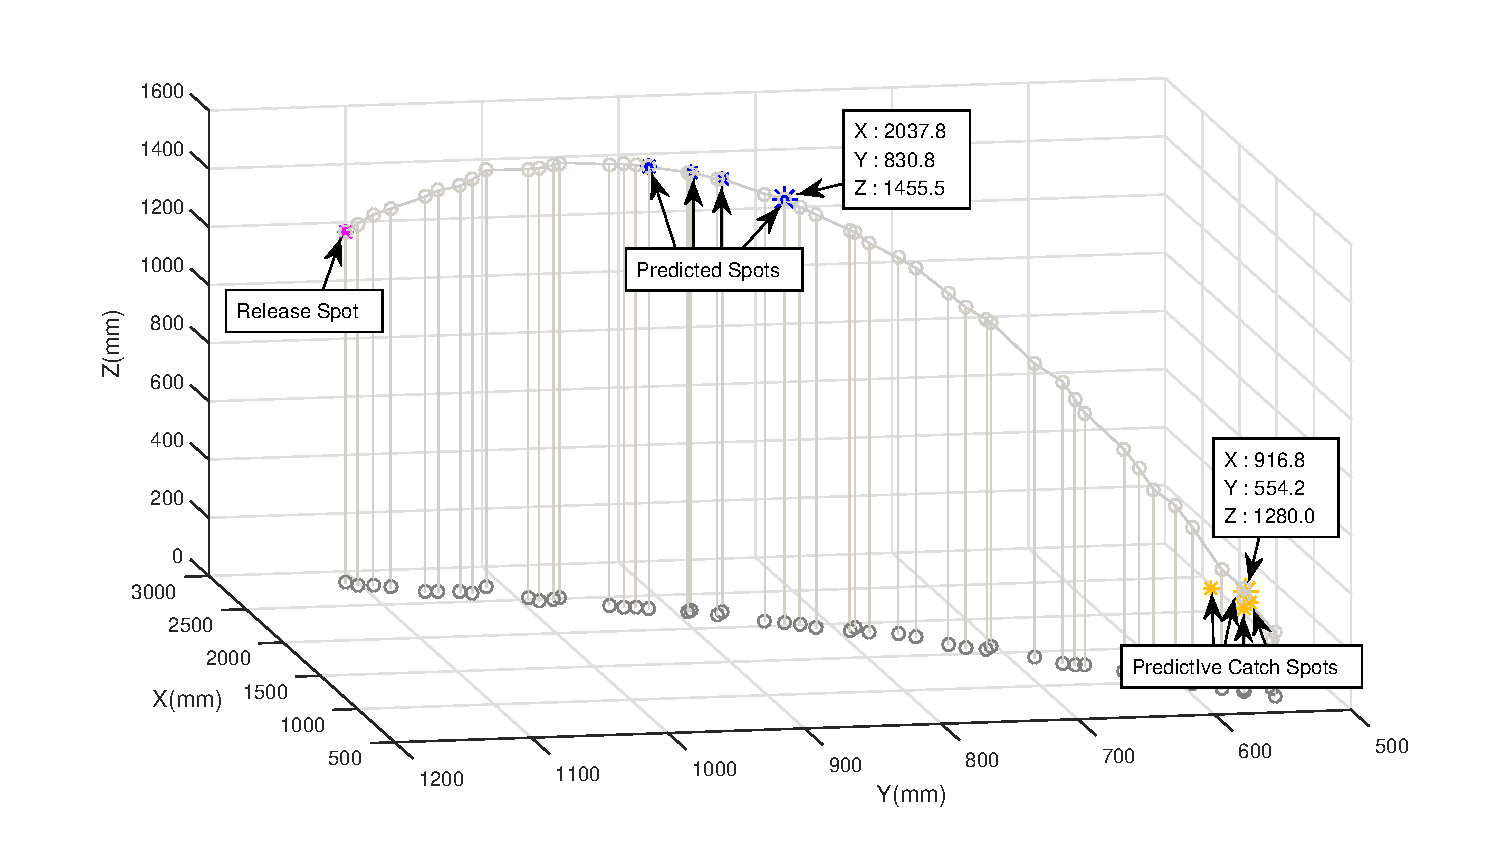
\includegraphics[width=3in]{fig/PFofRobot.eps}
		\caption{ Trajectory captured by the cameras. The red point denotes the position where the ball is thrown. The blue points are the positions where the catching points are predicted. The yellow points are the predictive catch points.}
		\label{fig:Trajectory}
	\end{figure}
	
	\subsection{Results of Case Two}
	The analysis of the two cases showed that the proposed $VCA$-based flexible structure provides a generic method to address the visual servo control problem in $ePLC$. Based on the $VCA$ protocol, the algorithms in the $VS$ and the $ePLC$ have a kind of normative correspondence, and the existing modules and motion control algorithms could be reused without additional programming. 
	\section{Conclusion}
	\label{conclusion}
	We proposed herein a flexible multi-level architecture based on the $VCA$ protocol to integrate the PLC, motion control, and visual systems. This architecture provides users an easy development method to ease the ever-growing complexity of applications. The multi-level architecture includes the flexible, control, and algorithm layers. The $VCA$ protocol is posed for data interaction among the layers. Correspondingly, customized hardware, memory allocation, and Petri-Net-based multithreading structure were described to support the proposed flexible software architecture. We implemented two cases, namely the winding machine with a visual system and the binocular catching robot, to illustrate the proposed system that provides a generic method to develop different types of applications of the visual servo system in $ePLC$. As a result, the proposed $VCA$-based architecture could easily be applied between two quite different cases.
	
	In a further research, we will implement a uniform development method of the visual servo control in the ePLC.
	
	\ifCLASSOPTIONcaptionsoff
	\newpage
	\fi
	
	
	
	% trigger a \newpage just before the given reference
	% number - used to balance the columns on the last page
	% adjust value as needed - may need to be readjusted if
	% the document is modified later
	%\IEEEtriggeratref{8}
	% The "triggered" command can be changed if desired:
	%\IEEEtriggercmd{\enlargethispage{-5in}}
	
	% references section
	
	% can use a bibliography generated by BibTeX as a .bbl file
	% BibTeX documentation can be easily obtained at:
	% http://www.ctan.org/tex-archive/biblio/bibtex/contrib/doc/
	% The IEEEtran BibTeX style support page is at:
	% http://www.michaelshell.org/tex/ieeetran/bibtex/
	%\bibliographystyle{IEEEtran}
	% argument is your BibTeX string definitions and bibliography database(s)
	%\bibliography{IEEEabrv,../bib/paper}
	%
	% <OR> manually copy in the resultant .bbl file
	% set second argument of \begin to the number of references
	% (used to reserve space for the reference number labels box)
	
	\bibliographystyle{IEEEtran}
	\bibliography{reference}
	
	% biography section
	%
	% If you have an EPS/PDF photo (graphicx package needed) extra braces are
	% needed around the contents of the optional argument to biography to prevent
	% the LaTeX parser from getting confused when it sees the complicated
	% \includegraphics command within an optional argument. (You could create
	% your own custom macro containing the \includegraphics command to make things
	% simpler here.)
	%\begin{IEEEbiography}[{\includegraphics[width=1in,height=1.25in,clip,keepaspectratio]{mshell}}]{Michael Shell}
	% or if you just want to reserve a space for a photo:
	
	%\begin{IEEEbiography}[{\includegraphics[width=1in,height=1.25in,clip,keepaspectratio]{fig/Author_HuifengWu.eps}}]{Huifeng Wu} received the Ph.D. degree in computer science and technology from Zhejiang university, Hangzhou, China, in 2006. He is currently a professor in the institute of intelligent and software Technology, Hangzhou Dianzi University. His research interests include software development methods and tools, software architecture, embedded system, intelligent control \& automation.
	%	
	%\end{IEEEbiography}
	%\begin{IEEEbiography}[{\includegraphics[width=1in,height=1.25in,clip,keepaspectratio]{fig/Author_YiYan.eps}}]{Yi Yan} received B.S. in automatic control engineering form Zhejiang Sci-Tech University in 1984, M.S. in computer engineering from Beijing University of Postal Telecommunications in 1990. Currently he is the director and full professor in institute of intelligent and software Technology, Hangzhou Dianzi University. His research interests include embedded system, advanced manufacturing system, intelligent control \& automation, and intelligent instruments.
	%	
	%	
	%\end{IEEEbiography}
	%\begin{IEEEbiography}[{\includegraphics[width=1in,height=1.25in,clip,keepaspectratio]{fig/Author_DanfengSun.eps}}]{Danfeng Sun} received M.S. in computer architecture from Hangzhou DianZi University in 2011. He is currently a research assistant in the Institute of Industrial Internet, Hangzhou DianZi University. His research interests include embeded system, motion control and IIoT.
	%\end{IEEEbiography}
	%\begin{IEEEbiography}[{\includegraphics[width=1in,height=1.25in,keepaspectratio,angle=-90]{fig/Author_ReneSimon.eps}}]{Rene Simon} obtained a doctor of engineering at the Otto-von-Guericke University Magdeburg in 2001. He is Professor of Control Systems at the Department of Automation and Computer Sciences, Harz University of Applied Sciences, Wernigerode, Germany. His major research fields include engineering of automation systems, especially industrial controllers. He is chairman of PLCopen and project leader IEC 61131-10 Ed. 1.0.
	%\end{IEEEbiography}
	
	
	
	% insert where needed to balance the two columns on the last page with
	% biographies
	%\newpage
	
	
	% You can push biographies down or up by placing
	% a \vfill before or after them. The appropriate
	% use of \vfill depends on what kind of text is
	% on the last page and whether or not the columns
	% are being equalized.
	
	%\vfill
	
	% Can be used to pull up biographies so that the bottom of the last one
	% is flush with the other column.
	%\enlargethispage{-5in}
	
	
	
	% that's all folks
\end{document}



